% Figure 1: the sequential detector, with the one component this paper changes.
% Compiled on its own (tectonic overview.tex) to overview.pdf.
\documentclass[tikz,border=2pt]{standalone}
\usepackage{times}
\usepackage{amsmath,amssymb,bm}
\usetikzlibrary{arrows.meta,positioning,calc,fit,backgrounds}
\begin{document}
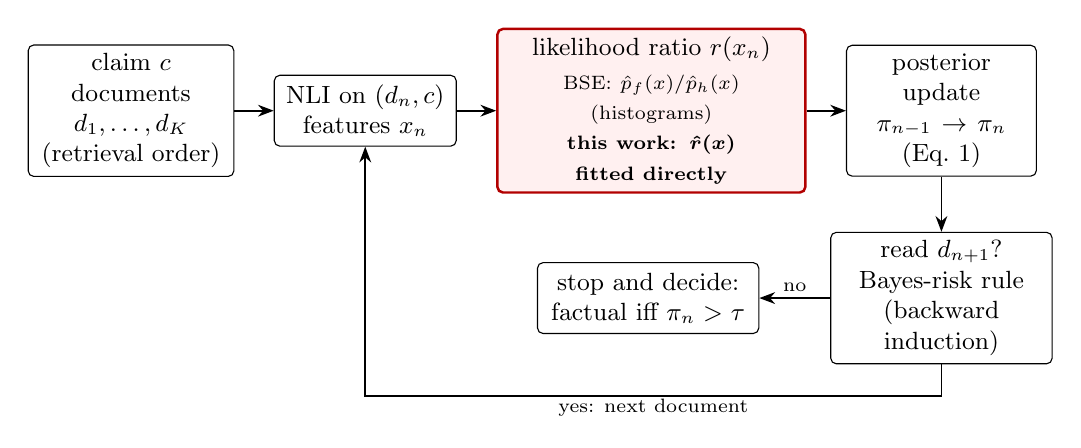
\begin{tikzpicture}[
  font=\small,
  box/.style={draw, rounded corners=2pt, align=center, minimum height=9mm,
              inner sep=3pt, fill=white},
  ours/.style={box, draw=red!70!black, fill=red!6, line width=0.9pt},
  flow/.style={-{Stealth[length=2mm]}, line width=0.6pt},
  lab/.style={font=\scriptsize, inner sep=1pt}]

\node[box, text width=24mm] (in) {claim $c$\\documents $d_1,\dots,d_K$\\(retrieval order)};
\node[box, text width=21mm, right=5mm of in] (nli) {NLI on $(d_n, c)$\\features $x_n$};
\node[ours, text width=37mm, right=5mm of nli] (ratio)
  {likelihood ratio $r(x_n)$\\[1pt]
   {\scriptsize BSE: $\hat p_f(x)/\hat p_h(x)$ (histograms)}\\
   {\scriptsize \textbf{this work: $\boldsymbol{\hat r(x)}$ fitted directly}}};
\node[box, text width=22mm, right=5mm of ratio] (upd) {posterior update\\$\pi_{n-1} \to \pi_n$ (Eq.~1)};
\node[box, text width=26mm, below=7mm of upd] (stop) {read $d_{n+1}$?\\Bayes-risk rule\\(backward induction)};
\node[box, text width=26mm, left=9mm of stop] (dec) {stop and decide:\\factual iff $\pi_n > \tau$};

\draw[flow] (in) -- (nli);
\draw[flow] (nli) -- (ratio);
\draw[flow] (ratio) -- (upd);
\draw[flow] (upd) -- (stop);
\draw[flow] (stop) -- node[lab, above=1pt] {no} (dec);
\draw[flow] (stop.south) -- ++(0,-4mm) -| node[lab, pos=0.25, below] {yes: next document}
  (nli.south);
\end{tikzpicture}
\end{document}
